\documentclass{Interspeech2024}

% 2023-10-21 modified by Simon King (Simon.King@ed.ac.uk)  

% 2024-01 modified by TPC Chairs of Interspeech 2024  

% **************************************
% *    DOUBLE-BLIND REVIEW SETTINGS    *
% **************************************
% Comment out \interspeechcameraready when submitting the 
% paper for review.
% If your paper is accepted, uncomment this to produce the
%  'camera ready' version to submit for publication.

%\interspeechcameraready 


% **************************************
% *                                    *
% *      STOP !   DO NOT DELETE !      *
% *          READ THIS FIRST           *
% *                                    *
% * This template also includes        *
% * important INSTRUCTIONS that you    *
% * must follow when preparing your    *
% * paper. Read it BEFORE replacing    *
% * the content with your own work.    *
% **************************************

% title here must exactly match the title entered into the paper submission system
\title{Paper Instructions and Template for Interspeech 2024}

% the order of authors here must exactly match the order entered into the paper submission system
% note that the COMPLETE list of authors MUST be entered into the paper submission system at the outset, including when submitting your manuscript for double-blind review
\name[affiliation={1,2}]{FirstNameA}{LastNameA}
\name[affiliation={3}]{FirstNameB}{LastNameB}
\name[affiliation={1,3}]{FirstNameC}{LastNameC}

%The maximum number of authors in the author list is 20. If the number of contributing authors is more than this, they should be listed in a footnote or the acknowledgement section.

% if you have too many addresses to fit within the available space, try removing the "\\" newlines
\address{
  $^1$First Affiliation, CountryX\\
  $^2$Second Affiliation, CountryY \\
  $^3$Third Affiliation, CountryZ}
\email{first@university.edu, second@companyA.com, third@companyB.ai}

\keywords{speech recognition, human-computer interaction, computational paralinguistics}

\newcommand{\red}[1]{\textcolor{red}{#1}}

\begin{document}

\maketitle

% the abstract here must exactly match the abstract entered into the paper submission system
\begin{abstract}
    
    % 1000 characters. ASCII characters only. No citations.
    Manuscripts submitted to Interspeech 2024 must use this document as both an instruction set and as a template. Do not use a past paper as a template. Always start from a fresh copy, and read it all before replacing the content with your own. The main changes with respect to previous instructions are \red{highlighted in red}.
    
    Before submitting, check that your manuscript conforms to this template. If it does not, it may be rejected. Do not be tempted to adjust the format! Instead, edit your content to fit the allowed space. The maximum number of manuscript pages is 5. The 5th page is reserved exclusively for \red{acknowledgements} and references, which may begin on an earlier page if there is space.
    
    The abstract is limited to 1000 characters. The one in your manuscript and the one entered in the submission form must be identical. Avoid non-ASCII characters, symbols, maths, italics, etc as they may not display correctly in the abstract book. Do not use citations in the abstract: the abstract booklet will not include a bibliography.  Index terms appear immediately below the abstract. 
\end{abstract}




\section{Introduction}

Templates are provided on the conference website for Microsoft Word\textregistered, and \LaTeX. We strongly recommend \LaTeX\xspace
which can be used conveniently in a web browser on \url{overleaf.com} where this template is available in the Template Gallery.

\subsection{General guidelines}

Authors are encouraged to describe how their work relates to prior work by themselves and by others, and to make clear statements about the novelty of their work. This may require careful wording to avoid unmasking the identity of the authors in the version submitted for review (guidance in Section \ref{section:doubleblind}). All submissions must be compliant with the ISCA Code of Ethics for Authors, the Pre-prints Policy, and the Conference Policy. These can be found on the conference website under the "For authors'' section.

\red{All (co-)authors must be responsible and accountable for the work and content of the paper, and they must consent to its submission. Generative AI tools cannot be a co-author of the paper. They can be used for editing and polishing manuscripts, but should not be used for producing a significant part of the manuscript.}


\subsubsection{Conference theme}

The theme of Interspeech~2024 is Speech and Beyond. Interspeech 2024 continues to be fully committed to advancing speech science and technology while meeting new challenges. Some of the intriguing topics that may be explored during this edition of Interspeech are Speech and Health, Animal Sound Recognition, Speech for interacting with Machines, Robots, and Apps (including VR/AR/XR), Speech for Memory and Heritage, and Communication across Ages.

\subsubsection{Author check list}

%Authors may wish to describe whether their work can be reproduced by others. 
The following checklist will be part of the submission form and includes a list of guidelines we expect Interspeech 2024 papers to follow. Not every point in the check list will be applicable to every paper. Ideally, all guidelines that do apply to a certain paper should be satisfied. Nevertheless, not satisfying a guideline that applies to your paper is not necessarily grounds for rejection. When your paper does not satisfy one or more of the guidelines in a section, the submission form will ask that you please explain why.

\begin{enumerate}

\item Claims and limitations - for all papers
\begin{itemize}

\item The paper clearly states what claims are being investigated.
\item The main claims made in the abstract and introduction accurately reflect the paper’s contributions and scope.
\item The limitations of your work are described.
\item All assumptions made in your work are stated in the paper.
 \end{itemize}

\item If data sets are used, the paper includes information about the following:
\begin{itemize}
\item Relevant details such as languages, audio duration distribution, number of examples, and label distributions, or a reference where that information can be found.
\item Details of train/validation (development)/test splits. Ideally, the lists should be released with the supplementary material if not already publicly available.
\item Explanation of all pre-processing steps, including any criteria used to exclude samples, if applicable.
\item Reference(s) to all data set(s) drawn from the existing literature.
\item For newly collected data, a complete description of the data collection process, such as subjects, instructions to annotators and methods for quality control and a statement on whether ethics approval was necessary.
\end{itemize}

\item If using non-public data sets:
\begin{itemize}
\item The paper includes a discussion on the reason/s for using non-public data sets.
\item Full details of the dataset are included in the paper to enable comparison to similar data sets and tasks.
\end{itemize}


\item If reporting experimental results, the paper includes:
\begin{itemize}
\item An explanation of evaluation metrics used.
\item An explanation of how models are initialized, if applicable.
\item \red{Some measure of statistical significance of the reported gains or confidence intervals (a python toolkit and brief tutorial for computing confidence intervals with the bootstrapping approach can be found in https://github.com/luferrer/ConfidenceIntervals).}
\item A description of the computing infrastructure used and the average runtime for each model or algorithm (e.g. training, inference etc).
\item The number of parameters in each model.
\end{itemize}

\item If hyperparameter search (including choice of architecture or features and any other development decision) was done, the paper includes:
\begin{itemize}
\item \red{Final results on a held-out evaluation set not used for hyperparameter tuning}.
\item Hyperparameter configurations for best-performing models.
\item The method for choosing hyperparameter values to explore, and the criterion used to select among them.
\end{itemize}

\item If source code is used:
\begin{itemize}
\item The code is or will be made publicly available and/or sufficient details are included in the paper for the work to be reproduced.
\item For publicly available software, the corresponding version numbers and links and/or references to the software.
\end{itemize}


\end{enumerate}


\subsection{Double-blind review}
\label{section:doubleblind}

Interspeech~2024 uses double-blind review to support the integrity of the review process. 

\subsubsection{Version submitted for review}

The manuscript submitted for review must not include any information that might reveal the authors' identities or affiliations. This also applies to the metadata in the submitted PDF file (guidance in Section \ref{section:pdf_sanitise}), uploaded multimedia and online material (guidance in Section \ref{section:multimedia}).
 
Take particular care to cite your own work in a way that does not reveal that you are also the author of that work. For example, do not use constructions like ``In previous work [23], we showed that \ldots''. Instead use something like ``Jones et al. [23] showed that \ldots''.
\red{Acknowledgements should not be included in the version submitted for review.}

%Authors who reveal their identity may be asked to provide a replacement manuscript. Papers for which a suitable replacement is not provided in a timely manner may be withdrawn.
Papers that reveal the identity of the authors will be rejected without review.
Note that the full list of authors must still be provided in the online submission system, since this is necessary for detecting conflicts of interest. 

\subsubsection{Camera-ready version}

Authors should include names and affiliations in the final version of the manuscript, for publication. \LaTeX\xspace users can do this simply by uncommenting  \texttt{\textbackslash interspeechcameraready}. The maximum number of authors in the author list is 20. If the number of contributing authors is more than this, they should be listed in a footnote or the Acknowledgements section. Include the country as part of each affiliation. Do not use company logos anywhere in the manuscript, including in affiliations and Acknowledgements. After acceptance, authors may of course reveal their identity in other ways, including: adjusting the wording around self-citations; adding further acknowledgements; updating multimedia and online material. Acknowledgements, if any, should be added in the camera-ready version.

\subsubsection{Pre-prints}
\label{section:preprints}

\red{Please, see \url{https://interspeech2024.org/submission-policy/} for a detailed explanation of the policy on pre-prints for this Interspeech. Note that this policy differs from that from priors years. The period of anonymity during which a version of the submitted paper may not be posted or updated online now starts a month before the Interspeech submission deadline and, as before, runs until accept/reject decisions are announced.}

%Authors should comply with the policy on pre-prints, which can be found on the conference website. Note that this policy applies not only to pre-prints (e.g., on arXiv) but also to other material being placed in the public domain that overlaps with the content of a submitted manuscript, such as blog posts. Do not make any reference to pre-print(s) -- including extended versions -- of your submitted manuscript. 
%Note that ISCA has a general policy regarding referencing publications that have not been peer-reviewed (Section \ref{section:references}). 


\section{Format}

\subsection{Layout}

Authors should observe the following specification for page layout by using the provided template. Do not modify the template layout! Do not reduce the line spacing!

\subsubsection{Page layout}

\begin{itemize}
\item Paper size must be DIN A4.
\item Two columns are used except for the title section and for large figures or tables that may need a full page width.
\item Left and right margin are \SI{20}{\milli\metre} each. 
\item Column width is \SI{80}{\milli\metre}. 
\item Spacing between columns is \SI{10}{\milli\metre}.
\item Top margin is \SI{25}{\milli\metre} (except for the first page which is \SI{30}{\milli\metre} to the title top).
\item Bottom margin is \SI{35}{\milli\metre}.
\item Text height (without headers and footers) is maximum \SI{235}{\milli\metre}.
\item Page headers and footers must be left empty.
\item No page numbers.
\item Check indentations and spacing by comparing to the example PDF file.
\end{itemize}

\subsubsection{Section headings}

Section headings are centred in boldface with the first word capitalised and the rest of the heading in lower case. Sub-headings appear like major headings, except they start at the left margin in the column. Sub-sub-headings appear like sub-headings, except they are in italics and not boldface. See the examples in this file. No more than 3 levels of headings should be used.

\subsubsection{Fonts}

Times or Times Roman font is used for the main text. Font size in the main text must be 9 points, and in the References section 8 points. Other font types may be used if needed for special purposes. \LaTeX\xspace users should use Adobe Type 1 fonts such as Times or Times Roman, which is done automatically by the provided \LaTeX\xspace class. Do not use Type 3 (bitmap) fonts. Phonemic transcriptions should be placed between forward slashes and phonetic transcriptions between square brackets, for example \textipa{/lO: \ae nd O:d3/} vs. \textipa{[lO:r@nO:d@]}, and authors are encouraged to use the terms `phoneme' and `phone' correctly \cite{moore19_interspeech}.


\subsubsection{Hyperlinks}

For technical reasons, the proceedings editor will strip all active links from the papers during processing. URLs can be included in your paper if written in full, e.g., \url{https://interspeech2024.org/speech-and-beyond/}. The text must be all black. Please make sure that they are legible  when printed on paper.


\subsection{Figures}

Figures must be centred in the column or page. Figures which span 2 columns must be placed at the top or bottom of a page.
Captions should follow each figure and have the format used in Figure~\ref{fig:speech_production}. Diagrams should preferably be vector graphics. Figures must be legible when printed in monochrome on DIN A4 paper; a minimum font size of  8 points for all text within figures is recommended. Diagrams must not use stipple fill patterns because they will not reproduce properly in Adobe PDF. Please use only solid fill colours in diagrams and graphs. All content should be viewable by individuals with colour vision deficiency (e.g., red-green colour blind) which can be achieved by using a suitable palette such one from \url{https://colorbrewer2.org} with the `colorblind safe' and `print friendly' options selected.


\subsection{Tables}

An example of a table is shown in Table~\ref{tab:example}. The caption text must be above the table. Tables must be legible when printed in monochrome on DIN A4 paper; a minimum font size of 8 points is recommended.

\begin{table}[th]
  \caption{This is an example of a table}
  \label{tab:example}
  \centering
  \begin{tabular}{ r@{}l  r }
    \toprule
    \multicolumn{2}{c}{\textbf{Ratio}} & 
                                         \multicolumn{1}{c}{\textbf{Decibels}} \\
    \midrule
    $1$                       & $/10$ & $-20$~~~             \\
    $1$                       & $/1$  & $0$~~~               \\
    $2$                       & $/1$  & $\approx 6$~~~       \\
    $3.16$                    & $/1$  & $10$~~~              \\
    $10$                      & $/1$  & $20$~~~              \\
    \bottomrule
  \end{tabular}
  
\end{table}


\subsection{Equations}

Equations should be placed on separate lines and numbered. We define
% 
\begin{align}
  x(t) &= s(t') \nonumber \\ 
       &= s(f_\omega(t))
\end{align}
% 
where \(f_\omega(t)\) is a special warping function. Equation \ref{equation:eq2} is a little more complicated.
% 
\begin{align}
  f_\omega(t) &= \frac{1}{2 \pi j} \oint_C 
  \frac{\nu^{-1k} \mathrm{d} \nu}
  {(1-\beta\nu^{-1})(\nu^{-1}-\beta)}
  \label{equation:eq2}
\end{align}
% 



\begin{figure}[t]
  \centering
  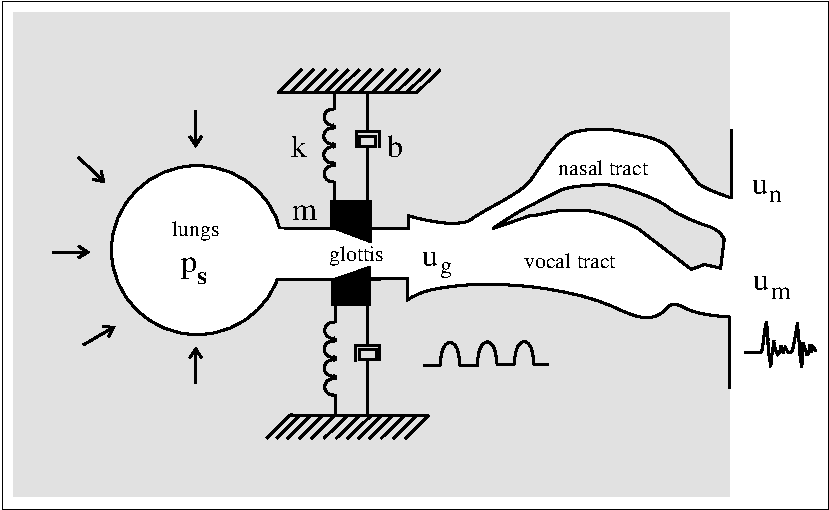
\includegraphics[width=\linewidth]{figure.pdf}
  \caption{Schematic diagram of speech production.}
  \label{fig:speech_production}
\end{figure}


\subsection{Style}

Manuscripts must be written in English. Either US or UK spelling is acceptable (but do not mix them).

\subsubsection{References}
\label{section:references}

It is ISCA policy that papers submitted to Interspeech should refer to peer-reviewed publications. References to non-peer-reviewed publications (including public repositories such as arXiv, Preprints, and HAL, software, and personal communications) should only be made if there is no peer-reviewed publication available, should be kept to a minimum, and should appear as footnotes in the text (i.e., not listed in the References). 

References should be in standard IEEE format, numbered in order of appearance, for example \cite{Davis80-COP} is cited before \cite{Rabiner89-ATO}. For longer works such as books, provide a single entry for the complete work in the References, then cite specific pages \cite[pp.\ 417--422]{Hastie09-TEO} or a chapter \cite[Chapter 2]{Hastie09-TEO}. Multiple references may be cited in a list \cite{Smith22-XXX, Jones22-XXX}.

\subsubsection{International System of Units (SI)}

Use SI units, correctly formatted with a non-breaking space between the quantity and the unit. In \LaTeX\xspace this is best achieved using the \texttt{siunitx} package (which is already included by the provided \LaTeX\xspace class). This will produce
\SI{25}{\milli\second}, \SI{44.1}{\kilo\hertz} and so on.


\begin{table}[b!]
  \caption{Main predefined styles in Word}
  \label{tab:word_styles}
  \centering
  \begin{tabular}{ll}
    \toprule
    \textbf{Style Name}      & \textbf{Entities in a Paper}                \\
    \midrule
    Title                    & Title                                       \\
    Author                   & Author name                                 \\
    Affiliation              & Author affiliation                          \\
    Email                    & Email address                               \\
    AbstractHeading          & Abstract section heading                    \\
    Body Text                & First paragraph in abstract                 \\
    Body Text Next           & Following paragraphs in abstract            \\
    Index                    & Index terms                                 \\
    1. Heading 1             & 1\textsuperscript{st} level section heading \\
    1.1 Heading 2            & 2\textsuperscript{nd} level section heading \\
    1.1.1 Heading 3          & 3\textsuperscript{rd} level section heading \\
    Body Text                & First paragraph in section                  \\
    Body Text Next           & Following paragraphs in section             \\
    Figure Caption           & Figure caption                              \\
    Table Caption            & Table caption                               \\
    Equation                 & Equations                                   \\
    \textbullet\ List Bullet & Bulleted lists                              \\\relax
    [1] Reference            & References                                  \\
    \bottomrule
  \end{tabular}
\end{table}


\section{Specific information for Microsoft Word}

For ease of formatting, please use the styles listed in Table \ref{tab:word_styles}. The styles are defined in the Word version of this template and are shown in the order in which they would be used when writing a paper. When the heading styles in Table \ref{tab:word_styles} are used, section numbers are no longer required to be typed in because they will be automatically numbered by Word. Similarly, reference items will be automatically numbered by Word when the ``Reference'' style is used.

If your Word document contains equations, you must not save your Word document from ``.docx'' to ``.doc'' because this will convert all equations to images of unacceptably low resolution.

\section{Submissions}

Information on how and when to submit your paper is provided on the conference website.

\subsection{Manuscript}

Authors are required to submit a single PDF file of each manuscript. The PDF file should comply with the following requirements: (a) no password protection; (b) all fonts must be embedded; (c) text searchable (do ctrl-F and try to find a common word such as ``the''). The conference organisers may contact authors of non-complying files to obtain a replacement. Papers for which an acceptable replacement is not provided in a timely manner will be withdrawn.

\subsubsection{Embed all fonts}

It is \textit{very important} that the PDF file embeds all fonts!  PDF files created using \LaTeX, including on \url{overleaf.com}, will generally embed all fonts from the body text. However, it is possible that included figures (especially those in PDF or PS format) may use additional fonts that are not embedded, depending how they were created. 

On Windows, the bullzip printer can convert any PDF to have embedded and subsetted fonts. On Linux \& MacOS, converting to and from Postscript will embed all fonts:
\\

\noindent\textsf{pdf2ps file.pdf}\\
\noindent\textsf{ps2pdf -dPDFSETTINGS=/prepress file.ps file.pdf}


\subsubsection{Sanitise PDF metadata}
\label{section:pdf_sanitise}

Check that author identity is not revealed in the PDF metadata. The provided \LaTeX\xspace class ensures this. Metadata can be inspected using a PDF viewer. 

\subsection{Optional multimedia files or links to online material}
\label{section:multimedia}

\subsubsection{Submitting material for inclusion in the proceedings}

Interspeech offers the option of submitting multimedia files. These files are meant for audio-visual illustrations that cannot be conveyed in text, tables and graphs. Just as with figures used in your manuscript, make sure that you have sufficient author rights to all other materials that you submit for publication. The proceedings will NOT contain readers or players, so be sure to use widely accepted formats, such as MPEG, WAVE PCM (.wav), and standard codecs.

Your multimedia files must be submitted in a single ZIP file for each separate paper. Within the ZIP file you can use folders to organise the files. In the ZIP file you should include a \texttt{README.txt} or \texttt{index.html} file to describe the content. In the manuscript, refer to a multimedia illustration by filename. Use short file names with no spaces.

The ZIP file you submit will be included as-is in the proceedings media and will be linked to your paper in the navigation interface of the proceedings. The organisers will not check that the contents of your ZIP file work.

Users of the proceedings who wish to access your multimedia files will click the link to the ZIP file which will then be opened by the operating system of their computer. Access to the contents of the ZIP file will be governed entirely by the operating system of the user's computer.

\subsubsection{Online resources such as web sites, blog posts, code, and data}

It is common for manuscripts to provide links to web sites (e.g., as an alternative to including a multimedia ZIP file in the proceedings), code repositories, data sets, or other online resources. Provision of such materials is generally encouraged; however, they should not be used to circumvent the limit on manuscript length. In particular, reviewers will not be required to read any content other than the main manuscript.

\red{Links included in the version submitted for review should not reveal the identity or affiliation of the authors. If this is not possible, then the links should not be provided in the version submitted for review, but they can be added in the final version of the paper, if accepted. A placeholder can be included in the paper with a text like: ``[to ensure author anonymity, the link to the resource will be added after the review process]''. }

%and a linked resource will inevitably reveal author identity, then authors should provide a warning to the reviewers, e.g., by linking to a special landing page that states `Clicking this link will reveal author identities'. 

\section{Discussion}

Authors must proofread their PDF file prior to submission, to ensure it is correct. Do not rely on proofreading the \LaTeX\xspace source or Word document. \textbf{Please proofread the PDF file before it is submitted.}


\section{Acknowledgements}
Acknowledgement should only be included in the camera-ready version, not in the version submitted for review.
The 5th page is reserved exclusively for \red{acknowledgements} and  references. No other content must appear on the 5th page. Appendices, if any, must be within the first 4 pages. The acknowledgments and references may start on an earlier page, if there is space.

\ifinterspeechfinal
     The Interspeech 2024 organisers
\else
     The authors
\fi
would like to thank ISCA and the organising committees of past Interspeech conferences for their help and for kindly providing the previous version of this template.


\bibliographystyle{IEEEtran}
\bibliography{mybib}

\end{document}
